\section{Introduction}

  I have yet to see any problem, however complicated, which, when looked at in the right way did not become still more complicated.

  \begin{flushright}--- Poul Anderson\end{flushright}

  People working in the field of high energy physics have a tendency to concern themselves with attempting to solve problems that are incredibly complicated.
  So, perhaps, there is a touch of irony that the problem that they are trying to solve is not only incredibly fundamental, but also very simple to state.
  The question can be boiled down to -- what is the stuff in our universe made of?
  What immediately follows from this fundamental inquiry is how is matter made up of these things ; or to put it another way, how do the fundamental building blocks interact.

  In some sense particle physics tries to distill matter and the interactions therein down to the smallest possible level to which it can be broken down.
  Turns out that breaking these concepts down to this elementary level of specificity is an incredibly complicated process of which we have merely begun to scratch the surface.  As such,this paper focuses on a tiny fraction of these fundamental building blocks -- the elusive neutrino with the hope of just perhaps being able to untangle some of the myriad of secrets that it harbours.

  \subsection{The Standard Model}

Before the protagonist
\footnote{Really the ensemble cast, given that they come in three flavors, electron($e\nu$), muon ($\mu \nu$) and tau($\tau \nu$)and their respective antiparticles,}
of our story - the neutrino - can be formally introduced, the stage has to be set.
A good candidate to set the stage would be the standard model which describes three of the four known fundamental forces, electromagnetic, weak and strong interactions (it struggles to deal with  gravity) and classifying all known elementary particles \cite{Oerter}.
Just like any foundational theory that undergirds a sub-field of a subject, the standard model definitely wasn't developed in a day and as such, there is definite value in becoming familliar with the historical context surrounding the standard model in our quest to understand neutrinos.

One may definitely quibble about where our understanding of the fundamental particles starts from, after all, humans have been trying to find out the nature of our universe and the things that make it up going back as far as the 4th century BCE with Plato positing that everything is made up of 4 elements (water, wind, earth and fire)\cite{Timaeus}, but I think it makes sense to look at the elementary particles that make up the standard model as we know it today -- with the definite understanding that there may very well be physics that lies beyond the realm of the standard model.

At its core, the Standard Model consists of two main categories of particles: fermions, which make up matter, and bosons, which mediate interactions.
Fermions have $1/2$ integer spins while bosons have integer spins \cite{Oerter}.

\begin{figure}[H]
  % 
  \centering
  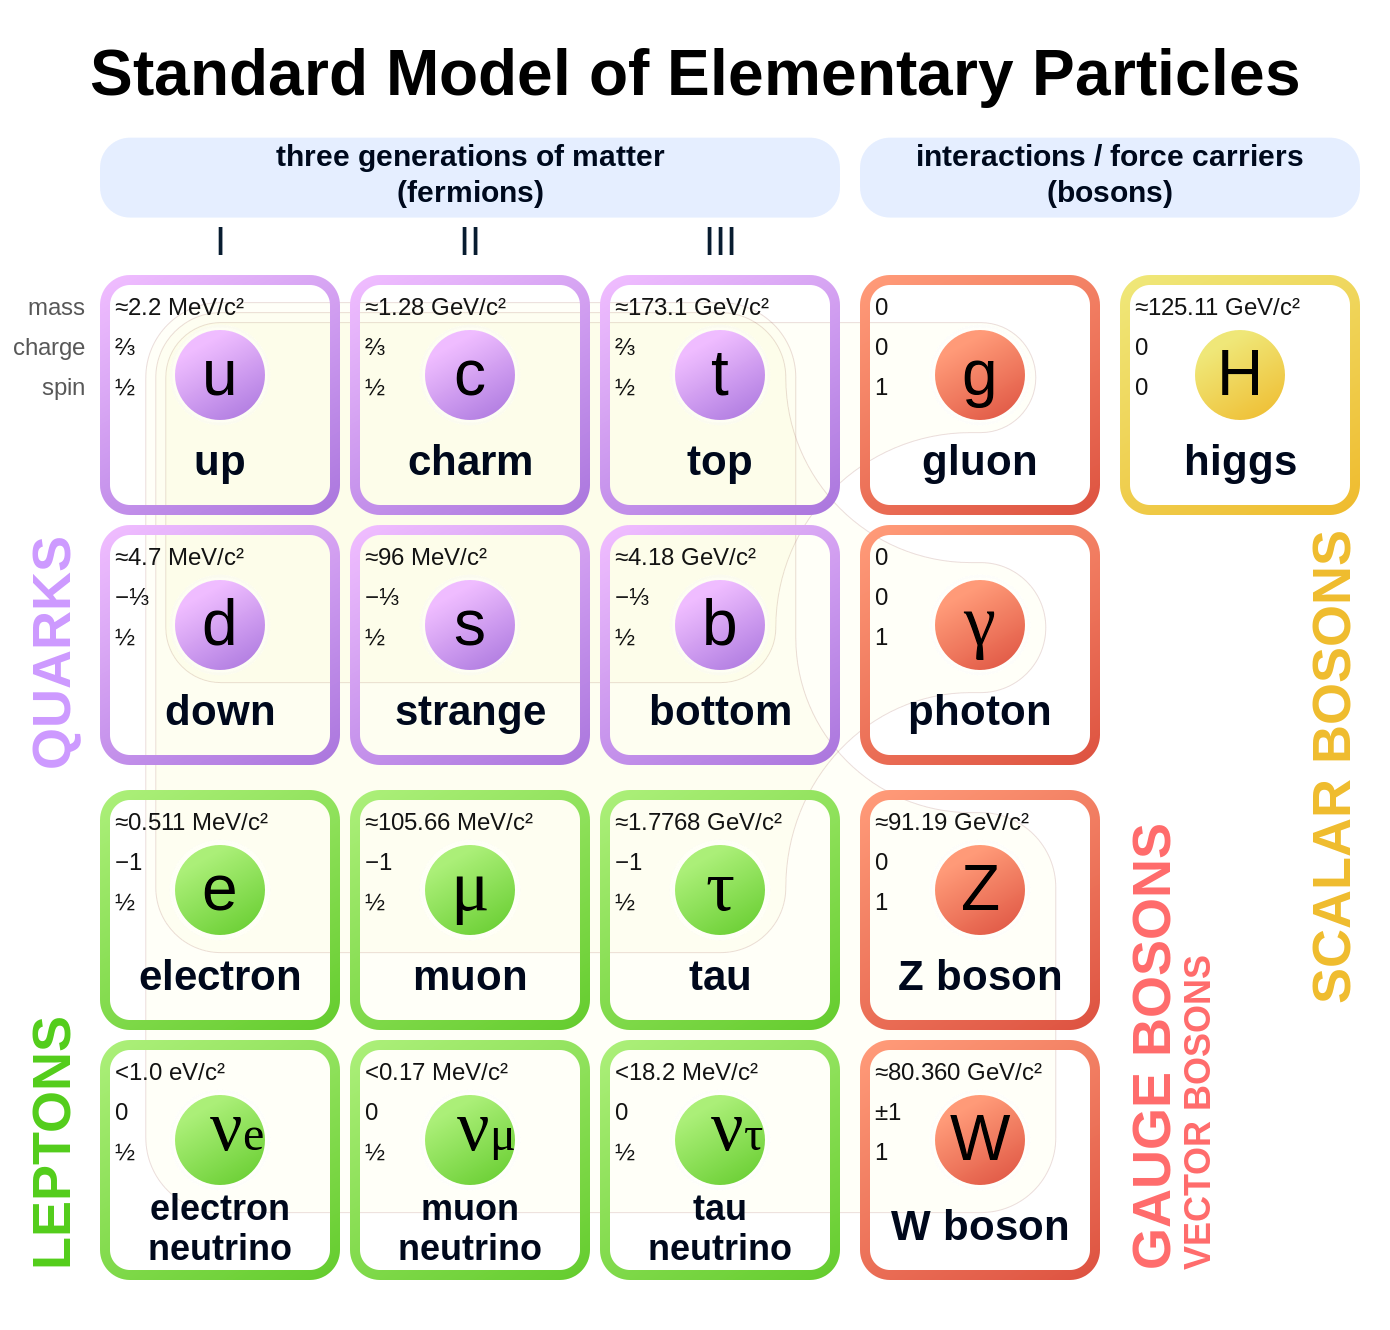
\includegraphics[width=80mm]{figures/sm.png}
  \caption{The Elementary Particles in the Standard Model \cite{standard_model}}
  \label{sm}
\end{figure}

The fermions can be further categorized into quarks and leptons.

\begin{figure}[H]
  % https://en.wikipedia.org/wiki/Quark#/media/File:Quark_structure_proton.svg
  \centering
  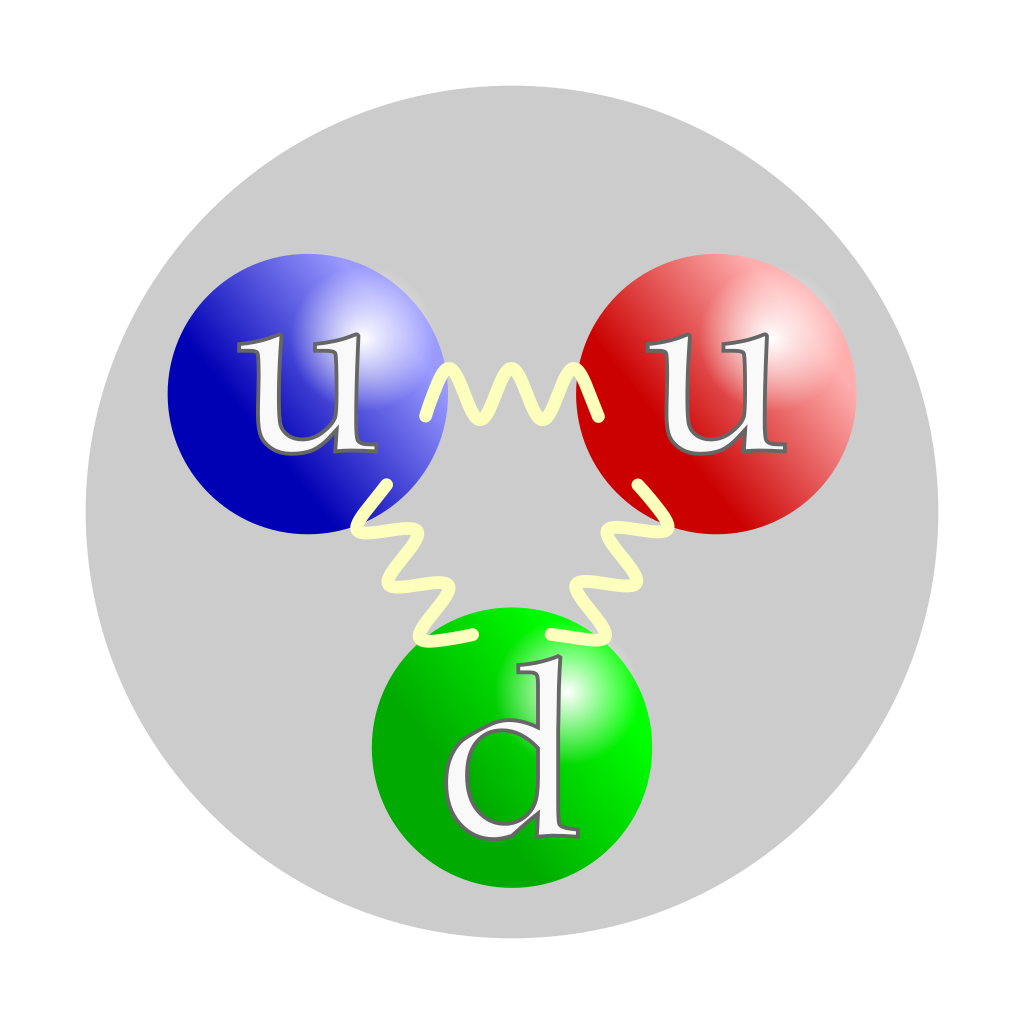
\includegraphics[width=100mm]{figures/protonQuarks.png}
  \caption{Quarks inside a proton.
    Labelled u for up and d for down\cite{quark}}
  \label{protonQuarks}
\end{figure}

Quarks are understood to be fundamental constituents of matter, forming the building blocks of protons, neutrons, and other hadrons (Composite subatomic particles that are made up of at least 2 quarks) \cite{quark_Brit_2024}.
Quarks interact with each other via the strong force.We have so far discovered 6 flavors of quarks -- up (\(u\)), down (\(d\)), charm (\(c\)), strange (\(s\)), top (\(t\)), and bottom (\(b\)).
Each flavor has different mass.
These masses and their interactions with other particles are crucial for the stability and properties of atomic nuclei \cite{Nave_quark}.

\begin{table}[h!]

  \centering
  \begin{tabular}{lrr}
    \toprule
    Quark Flavor & Approximate Mass (MeV/c\(^2\)) & Charge (e) \\
    \midrule
    Up (u)      & 2.2 - 3.0        & +\(\frac{2}{3}\) \\
    Down (d)    & 4.7 - 5.0        & -\(\frac{1}{3}\) \\
    Strange (s) & 95 - 105         & -\(\frac{1}{3}\) \\
    Charm (c)   & 1270 - 1720      & +\(\frac{2}{3}\) \\
    Bottom (b)  & 4180 - 4380      & -\(\frac{1}{3}\) \\
    Top (t)     & 172000 - 173000  & +\(\frac{2}{3}\) \\
    \bottomrule
  \end{tabular}
  \caption{Quark Flavors, Their Approximate Masses and Charges \cite{Nave_quark}}
  \label{quarkMass}
\end{table}

Each type of fermion carries a specific flavor and generation.
For instance, the electron ($e$) belongs to the first generation, while the muon ($\mu$) and tau ($\tau$) belong to the second and third generations, respectively \cite{Nave_lepton} \footnote{The neutrino, despite being elusive, plays a significant role in weak interactions and lepton family conservation.}.

The interactions between these particles are mediated by gauge bosons, which are the force carriers \cite{Gribbin_2000}\cite{Clark_2004}.
The Standard Model includes the following gauge bosons:

\begin{align}
 & \quad \text{Photon } (\gamma) \quad \text{(mediates electromagnetic force)} \\
                    & \quad \text{W and Z bosons } (W^\pm, Z^0) \quad \text{(mediates weak force)} \\
                    & \quad \text{Gluons } (g) \quad \text{(mediates strong force) \cite{Veltman_2004}}
\end{align}

The mathematical framework underpinning the Standard Model is primarily based on gauge theory, specifically the group $SU(3) \times SU(2) \times U(1)$.
Each of these groups corresponds to a different force:

\begin{align}
\text{Strong Interaction:} & \quad SU(3) \quad \text{(color charge)} \\
\text{Weak Interaction:} & \quad SU(2) \quad \text{(isospin)} \\
\text{Electromagnetic Interaction:} & \quad U(1) \quad \text{(hypercharge)}
\end{align}

The Higgs mechanism, a crucial part of the Standard Model, provides a mass to the W and Z bosons via spontaneous symmetry breaking.
The Higgs field $\phi$ can be parameterized as:

\begin{align}
\phi &= \frac{v+h}{\sqrt{2}}e^i{\frac{\chi}{v}}
\end{align}

where $h$, the Higgs boson and $\chi$, the Goldstone boson are real scalar fields which have no vacuum expectation value.
The mass terms for the gauge bosons arise when the Higgs field acquires a vacuum expectation value\cite{Bernardi_2008}.



  \subsection{The Electron}

For the longest time, humans had thought that atoms were the smallest particle that makes up everything in the world and cannot be subdivided further\cite{Dalton}, but this idea had started to come under scrutiny by the late 1800's\cite{Pullman}.
Even then, it was thought that if anything were to make up atoms, they wouldn't be lighter than the lightest atom \cite{Thorpe}.
However, in 1897, Thomson would come in with evidence that there not only were particles that made up the atoms, but that they were on the scale of 1000 times lighter than hydrogen\cite{Thomson_1907}.
He decided to shoot cathode rays at a thermal junction so he could measure the generated heat and measured how much they deflected magnetically.
He also measured the electrical deflections by lowering the pressure in the chamber where he was measuring the deflection\cite{Thomson}.
Through these experiments, he discovered the electron
\footnote{Although Thomson did decide to call them corpuscles; a name which definitely did not stick around}
and believed that it was a fundamental part of all atoms that was very light and held a decidedly negative charge\cite{electronDiscovery}.



  \subsection{Dalton's Atomic Theory}

The discovery of something so much smaller than the lightest atom threw Dalton's atomic theory out the window.
His theory claimed that  everything in the universe was made up of atoms which would vary in size and mass based on the element.
These atoms could not be created or destroyed, but  could reaarrange themselves through chemical reactions.
It could be argued that Dalton's model was a progenitor for the idea of conservation of mass and energy.
Despite being such an important idea, even before the discovery of electrons, the theory wasn't fullproof; it could not account for isotopes of the same element having different masses, but the electron blew the idea wide apart.

A new theory that looked at the atom not as the smallest thing that could exist but rather something that had other things inside in some sort of structure had to be developed.


  \subsection{The Plum Pudding Model}

There were numerous models that tried to tackle this problem and one of the first was proposed by Thompson in 1904 as the plum pudding model.
The first problem to grapple with was that electrons are negatively charged while the atoms themselves are electrically neutral.
To get around this, the plum pudding model suggests that  the electrons were suspended in a morass of positively charged particles
\footnote{Kind of like plums suspended in a pudding, hence the name of the model}
with the charge between the positive  and negative equalling out to 0.
Thomson believed that the mass was evenly distributed throughout the atom.

\begin{figure}[H]
  % https://en.m.wikipedia.org/wiki/File:Plum_pudding_atom.svg
  \centering
  
\includegraphics[width=100mm]{figures/plumPudding.png}
  \caption{Cartoon of plum pudding model}
  \label{plumPudding}
\end{figure}

The plum pudding model struggled to explain how these charged particles were so copacetic with each other despite being such small physical distances apart.
It was well known by then that opposite charges attract while alike charges repel.
It also failed to provide any explanation of the spectral lines observed in hydrogen.
Darker clouds were still on the horizon for Thomson's plum pudding model.


  \subsection{Gold Foil Experiments}

Between 1908 and  1913, a number of alpha ($\alpha$) particle scattering experiments were performed by Hans Geiger and Ernest Marsden.
These took the form of shooting $\alpha$  particles at a  incredibly thin piece of gold foil.
Based on the plum pudding model, it was expected that the $\alpha$ particles would not be deflected however this turned out not to be the case at all.
To be fair, most of the $\alpha$ particles did indeed go straight through the gold foil, their trajectory not disturbed in the slightest.
A smaller fraction did get deflected, some by a small angle and others by a large one.
But the astonishing part was that an even smaller fraction, about 1 in 20000, shot right back at the direction the particle gun was shooting from.

\begin{figure}[H]
  % https://en.wikipedia.org/wiki/Rutherford_scattering_experiments#/media/File:Geiger-Marsden_experiment_expectation_and_result.svg
  \centering
  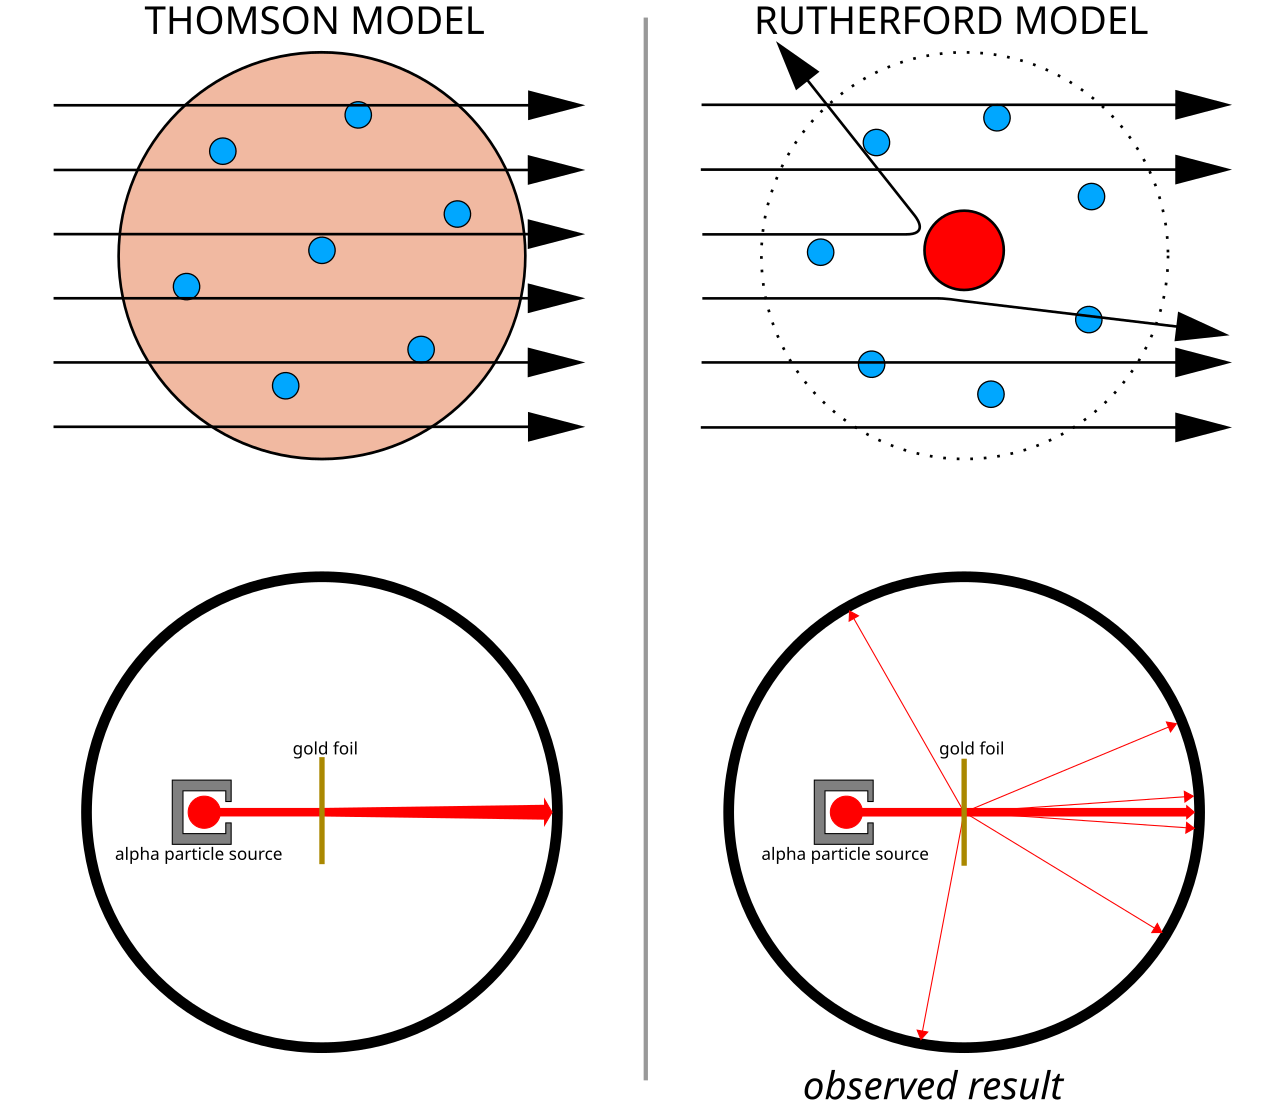
\includegraphics[width=100mm]{figures/goldFoil.png}
  \caption{Cartoon of Gold foil experiment}
  \label{goldFoil}
\end{figure}



  \subsection{Rutherford's Model}

So a new model was required to explain the discrepencies away; in comes Rutherford.
He looked at the gold foil experiments done before him and ran with it, expanding upon them and developing a new theory on the substructure of the atom.
He proposed in 1911 that atoms were mostly just empty spacewith a highly concentrated segment of mass at the center of the atom -- he called this central mass the neucleus of the atom.
In Rutherford's atomic model, the electrons orbit around the positively charged neucleus.

\begin{figure}[H]
  % https://en.wikipedia.org/wiki/Rutherford_model#/media/File:Rutherford_atomic_planetary_model.svg
  \centering
  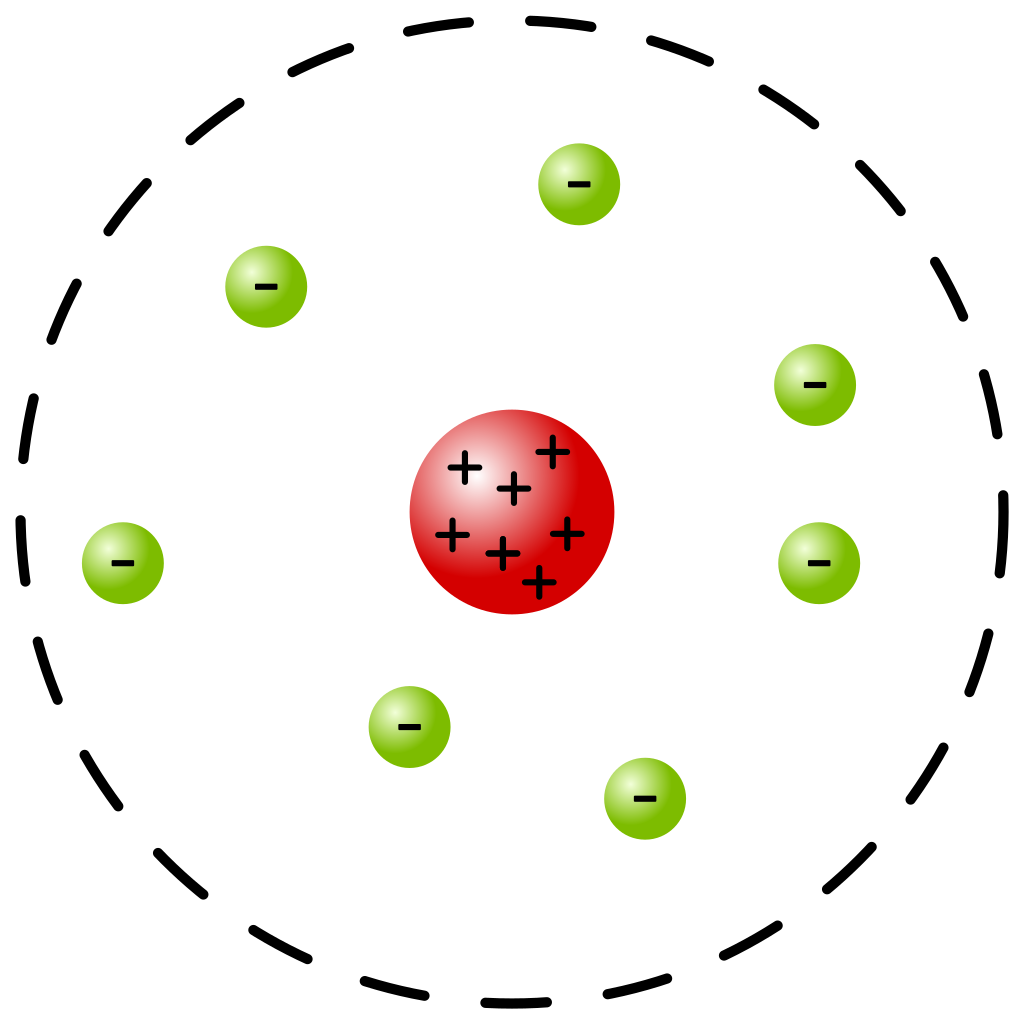
\includegraphics[width=100mm]{figures/rutherford.png}
  \caption{Rutherford's atomic model}
  \label{rutherford}
\end{figure}

Only, one little problem.
When things move in a circular orbit, they are accelerating and when a charged particle is moving in an orbit like that,  it should be constantly radiating energy leading to it eventually falling into the neucleus rendering this formulation of the atom unstable.
It should also be emitting a continous energy spectrum from the electrons, but hydrogen has discrete spectral lines.



  \subsection{Bohr's Model}

Bohr tried to come at this from an angle that resolved the spectral line issue with Rutherford's model.
Bohr proposed that electrons move in fixed orbits, thus explaining the discrete lines of the hydrogen spectra and that atoms emit light when an electron jumps from a higher energy level to a lower one.

\begin{figure}[H]
  % https://en.wikipedia.org/wiki/Bohr_model#/media/File:Bohr_atom_model.svg 
  \centering
  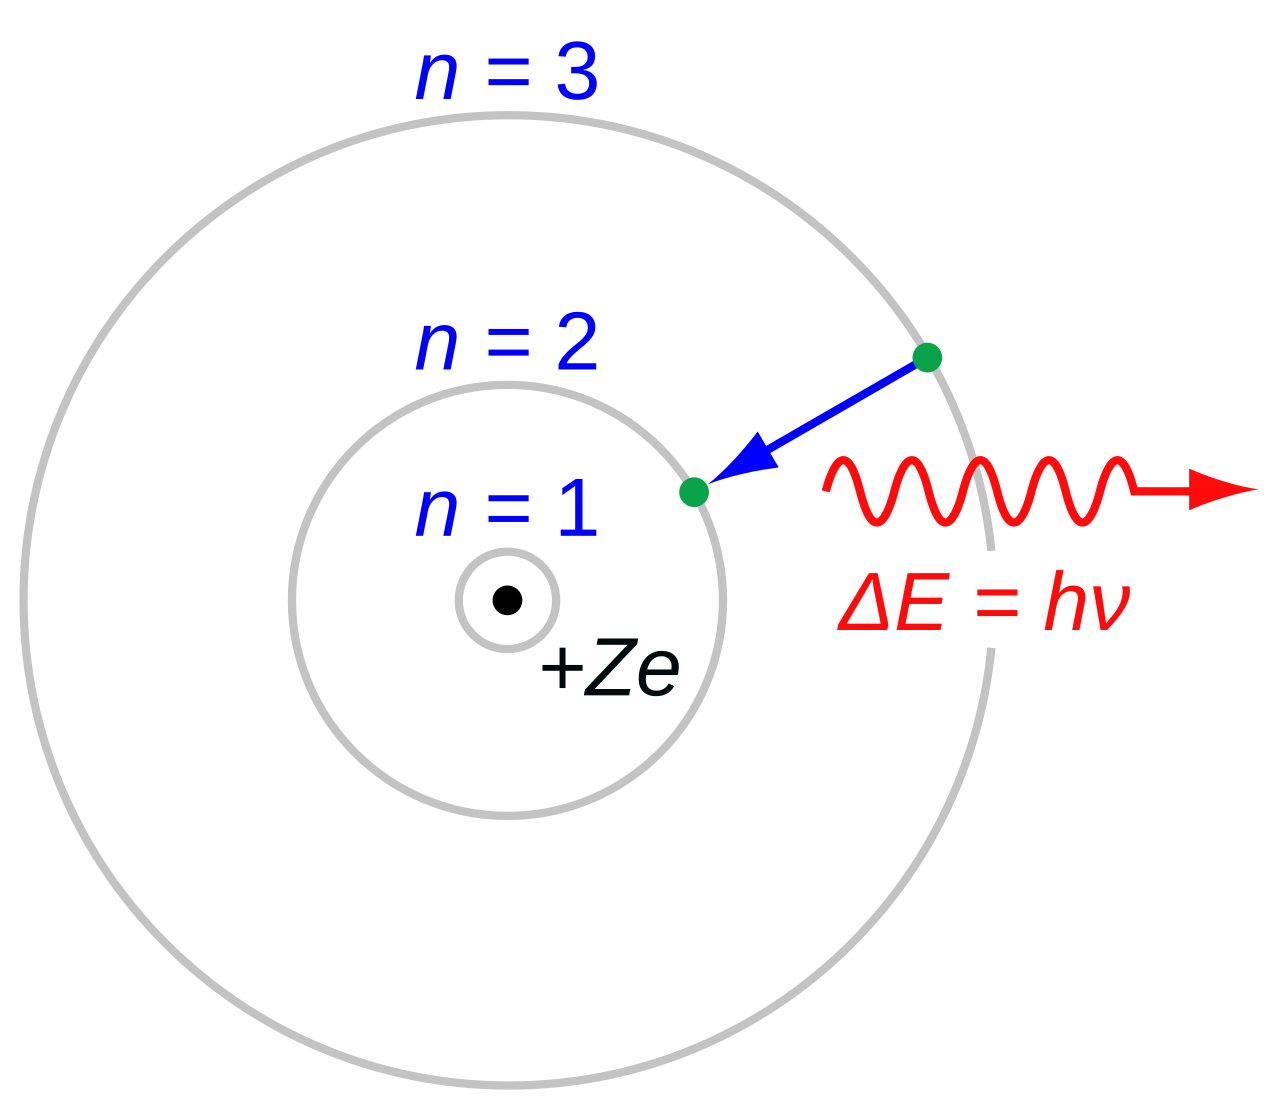
\includegraphics[width=100mm]{figures/bohr.png}
  \caption{Bohr's model of the hydrogen atom}
  \label{bohr}
\end{figure}

This still doesn't explain away why the electron doesn't collapse into the neucleus .
However, it does a very good job of modelling hydrogen and hydrogen-like atoms under most normal conditions.
The other issue with Bohr's model is that it fails to adress De-Broglie’s Hypothesis of the dual nature of matter..
To get there, we have to delve into the wonderful world of quantum mechanics.


  \subsection{Electroweak Interactions}